\begin{proofbox}
  \textbf{\textcolor{CProof}{证明一｜指数反推法（门槛最低）}}

  \textbf{从哪里想起？}对数本来就是指数的另一种写法。设 $x=\log_a b$，即 $a^x=b$；只要判断“为了得到 $b$，指数 $x$ 应取正还是负”。
  \begin{description}[style=nextline,leftmargin=2.4em,labelsep=0.45em,itemsep=0.35em]
    \item[第一步：$a>1$。]由于 $a^0=1$，当 $x>0$ 时 $a^x>1$，当 $x<0$ 时 $0<a^x<1$。因此 $b>1$ 对应 $x>0$；$0<b<1$ 对应 $x<0$。
    \item[第二步：$0<a<1$。]当 $x>0$ 时 $0<a^x<1$，当 $x<0$ 时 $a^x>1$。因此 $0<b<1$ 对应 $x>0$；$b>1$ 对应 $x<0$。
    \item[第三步：合并。]正好是底数、真数位于 $1$ 同侧时 $x>0$，异侧时 $x<0$。又 $a^0=1$，所以 $b=1$ 时 $x=0$。
  \end{description}
  \begin{center}
  \begin{tikzpicture}[font=\small,>=stealth,every node/.style={align=center,text width=5.6cm,inner sep=7pt}]
    \node[draw,rounded corners,fill=teal!8] (aa) at (0,0) {$2^2=4$\\$\Rightarrow \log_2 4=2>0$};
    \node[draw,rounded corners,fill=orange!9] (ab) at (6.5,0) {$2^{-2}=\frac14$\\$\Rightarrow \log_2\frac14=-2<0$};
    \node[draw,rounded corners,fill=teal!8] (ba) at (0,-1.9) {$(\frac12)^2=\frac14$\\$\Rightarrow \log_{\frac12}\frac14=2>0$};
    \node[draw,rounded corners,fill=orange!9] (bb) at (6.5,-1.9) {$(\frac12)^{-2}=4$\\$\Rightarrow \log_{\frac12}4=-2<0$};
    \node[above,teal!70!black] at (aa.north) {同侧：正};
    \node[above,orange!80!black] at (ab.north) {异侧：负};
  \end{tikzpicture}

  \end{center}

  \medskip
  \textbf{\textcolor{CProof}{证明二｜函数图像法（最直观）}}

  \textbf{从哪里想起？}对数的正负，就是图像位于 $x$ 轴上方还是下方。
  \begin{description}[style=nextline,leftmargin=2.4em,labelsep=0.45em,itemsep=0.35em]
    \item[第一步：找分界点。]两个函数 $y=\log_a x$ 都经过 $(1,0)$，因为 $\log_a1=0$。
    \item[第二步：看增减。]当 $a>1$ 时图像从左向右上升；因此 $x>1$ 时函数值为正，$0<x<1$ 时为负。当 $0<a<1$ 时图像下降，正负刚好倒过来。
    \item[第三步：把 $x$ 换成 $b$。]得到四种情况，与证明一相同。
  \end{description}
  \begin{center}
  \begin{tikzpicture}[x=.74cm,y=.72cm,>=stealth]
    \begin{scope}
      \draw[->] (0,-1.7)--(0,1.95) node[above] {$y$}; \draw[->] (0,0)--(4.55,0) node[right] {$x$};
      \draw[thick,teal!75!black,samples=80,domain=.3:4.2] plot (\x,{ln(\x)/ln(2)});
      \fill (1,0) circle (2pt); \node[below right] at (1,0) {$1$};
      \node at (2.8,2.75) {$a>1$}; \node[teal!75!black] at (2.7,.7) {$+$}; \node[orange!85!black] at (.53,-1.85) {$-$};
    \end{scope}
    \begin{scope}[shift={(6.3,0)}]
      \draw[->] (0,-1.7)--(0,1.95) node[above] {$y$}; \draw[->] (0,0)--(4.55,0) node[right] {$x$};
      \draw[thick,orange!80!black,samples=80,domain=.3:4.2] plot (\x,{-ln(\x)/ln(2)});
      \fill (1,0) circle (2pt); \node[above right] at (1,0) {$1$};
      \node at (2.8,2.75) {$0<a<1$}; \node[teal!75!black] at (.75,1.5) {$+$}; \node[orange!85!black] at (2.7,-.7) {$-$};
    \end{scope}
  \end{tikzpicture}

  \end{center}

  \medskip
  \textbf{\textcolor{CProof}{证明三｜换底公式法（计算题好用）}}

  \textbf{从哪里想起？}把不同底数的对数统一改写成以 $2$ 为底，就不用分别讨论原底数了。
  \begin{description}[style=nextline,leftmargin=2.4em,labelsep=0.45em,itemsep=0.35em]
    \item[第一步：换底。]由换底公式
      \[\log_a b=\frac{\log_2 b}{\log_2 a}.\]
      因为 $a\neq1$，所以分母 $\log_2 a\neq0$。
    \item[第二步：分别判号。]由于底数 $2>1$，$\log_2 t$ 与 $t-1$ 正负相同（$t>0$）；因此分子和 $b-1$ 同号，分母和 $a-1$ 同号。
    \item[第三步：看分式正负。]分子与分母同号时分式为正，异号时为负。故
      \[\boxed{\ \log_a b>0\iff(a-1)(b-1)>0\ },\qquad
        \boxed{\ \log_a b<0\iff(a-1)(b-1)<0\ }.\]
      $b=1$ 时分子是 $0$，所以对数为 $0$。
  \end{description}
  \begin{center}
  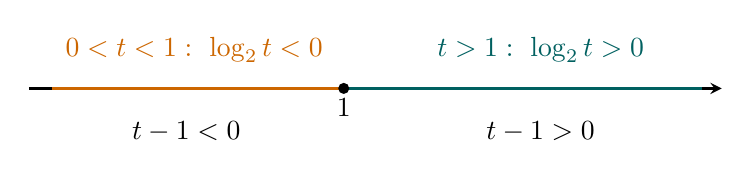
\begin{tikzpicture}[x=1cm,y=1cm,>=stealth]
    \draw[->,thick] (.2,0)--(9.0,0);
    \draw[very thick,orange!80!black] (.5,0)--(4.2,0);
    \draw[very thick,teal!75!black] (4.2,0)--(8.75,0);
    \fill (4.2,0) circle (2pt) node[below] {$1$};
    \node[above,orange!80!black] at (2.3,.2) {$0<t<1:\ \log_2t<0$};
    \node[above,teal!75!black] at (6.7,.2) {$t>1:\ \log_2t>0$};
    \node[below] at (2.2,-.3) {$t-1<0$};
    \node[below] at (6.7,-.3) {$t-1>0$};
  \end{tikzpicture}

  \end{center}
  \textbf{\textcolor{CProof}{三种证明的共同关键：}}$1$ 是分界点；无论哪种办法，都是在比较底数和真数分别处于 $1$ 的哪一侧。
\end{proofbox}
